\documentclass{beamer}
\usepackage[british]{babel}
\usepackage[utf8]{inputenc}
\usepackage{styles/jyumacros}
\usepackage{hyperref}
\usepackage{caption}
\usepackage{subcaption}
\usepackage[absolute,overlay]{textpos}
\usepackage[texcoord]{eso-pic}
\setbeamertemplate{caption}[​numbered]
\usefolder{styles}
\usetheme{jyu}
\titlegraphic{assets/coverlogo.pdf}
\newcommand{\smalllogo}{assets/small_white.pdf}
\graphicspath{{./assets/}}

\title{Current Status of MARA-LEB}
\date{29.06.2021}
\author[auth]{Jorge Romero}

\begin{document}
\begin{frame}
\titlepage
\end{frame}
\begin{frame}{RFQ}
    \begin{textblock*}{0.5\textwidth}(0.1\textwidth,0.3\textheight)
    \centering
    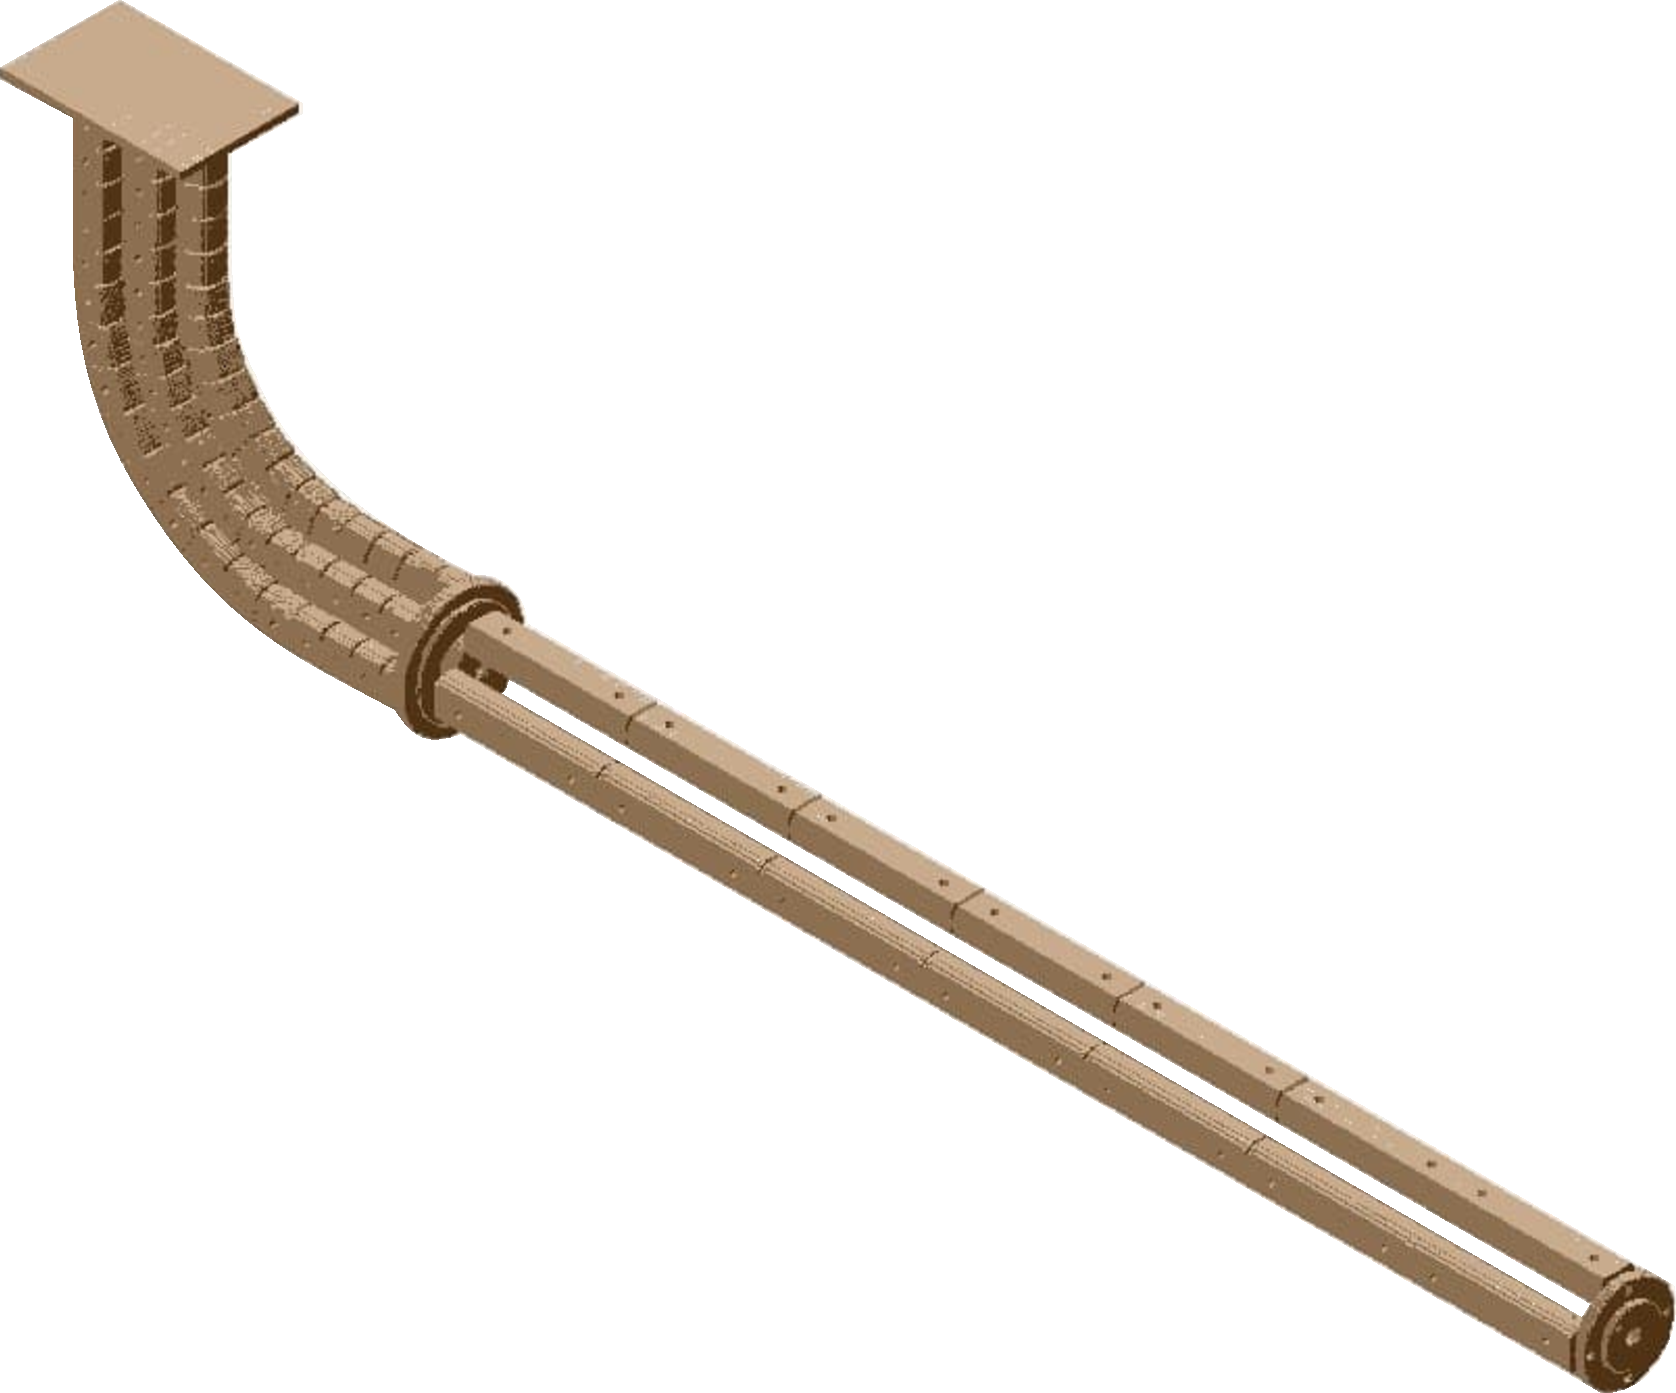
\includegraphics[scale=0.25]{RFQ.pdf}
    \end{textblock*}
    \begin{textblock*}{0.7\textwidth}(0.35\textwidth,0.55\textheight)
        \begin{itemize}
            \item \textbf{Aperture between vacuum chambers}
        \end{itemize}
    \end{textblock*}
\end{frame}
\begin{frame}{Transmission}
    \vspace*{2em}
    \centering
    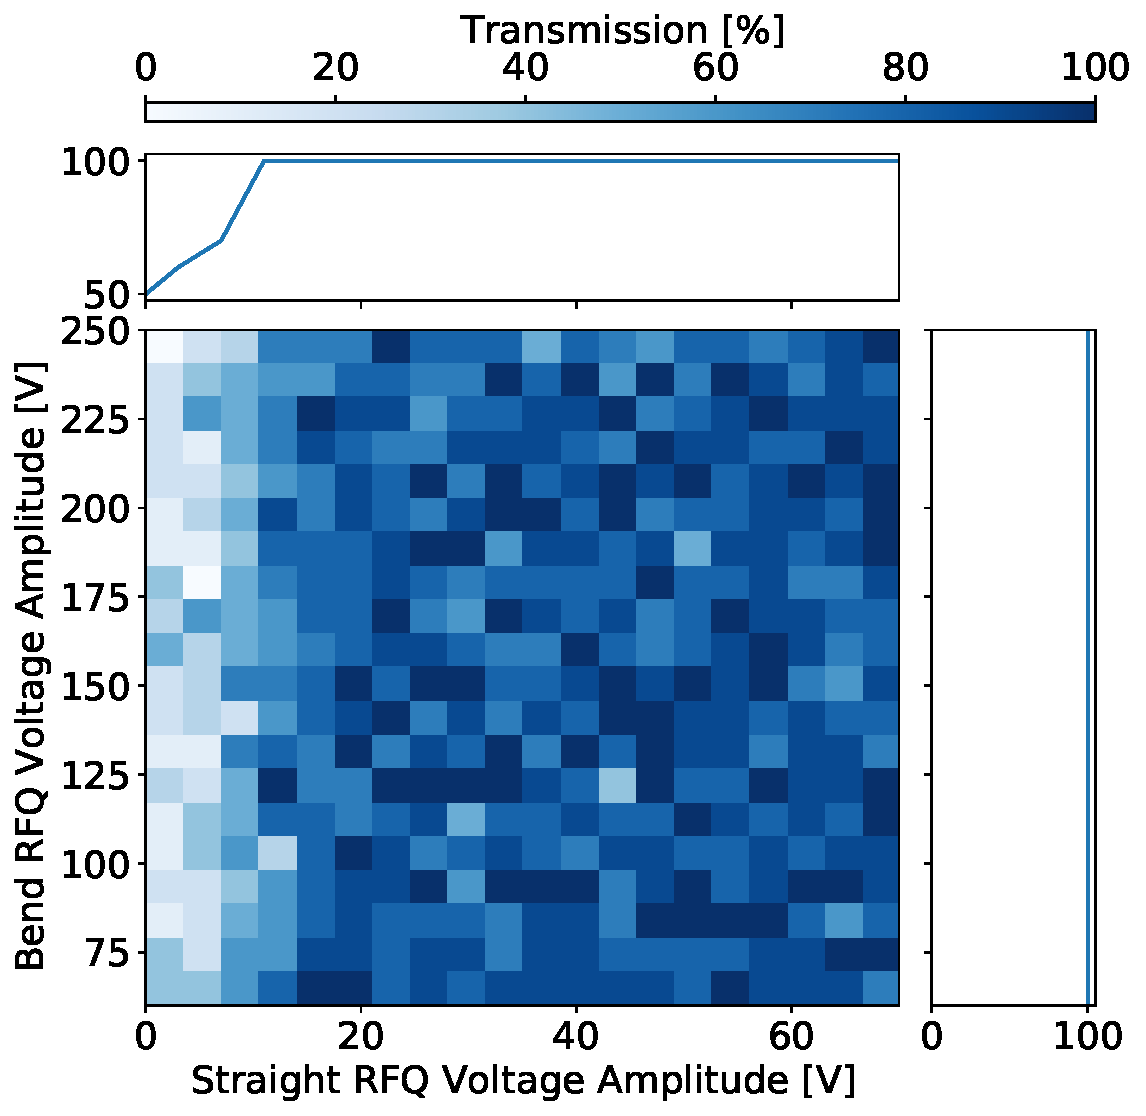
\includegraphics[scale=0.4]{gas_2cham.pdf}
\end{frame}
\begin{frame}{Losses}
    \vspace*{2em}
    \centering
    \hspace*{-2em}
    \includegraphics<1>[width=1.1\textwidth]{splats2cham.pdf}
    % \includegraphics<2>[width=1.1\textwidth]{splats1cham.pdf}
\end{frame}
\begin{frame}{Electrode Design}
    \vspace*{2.5em}
    \begin{figure}
        \centering
        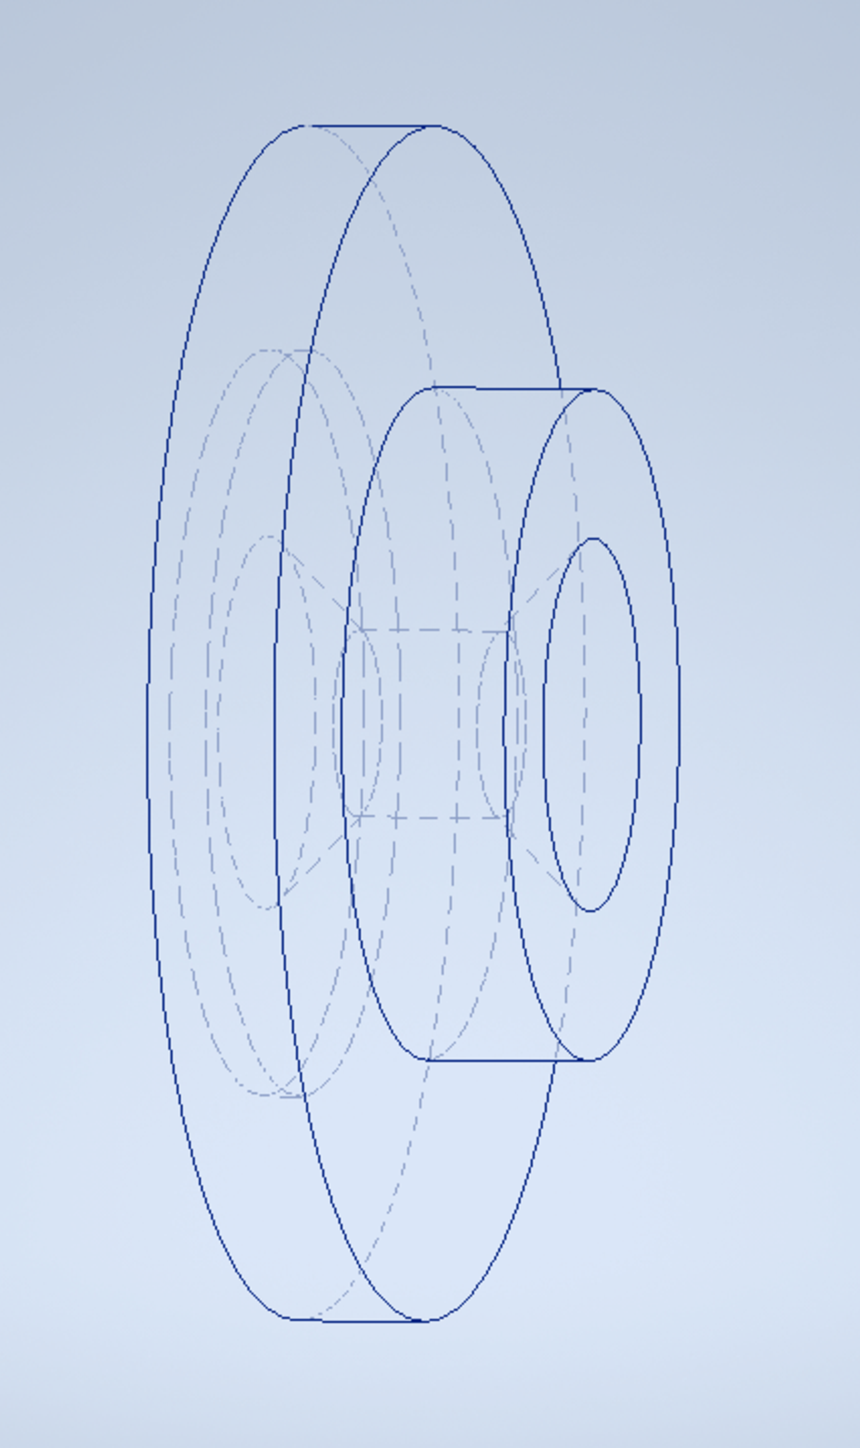
\includegraphics[scale=0.2]{oldchamfer.pdf}\hspace*{1em}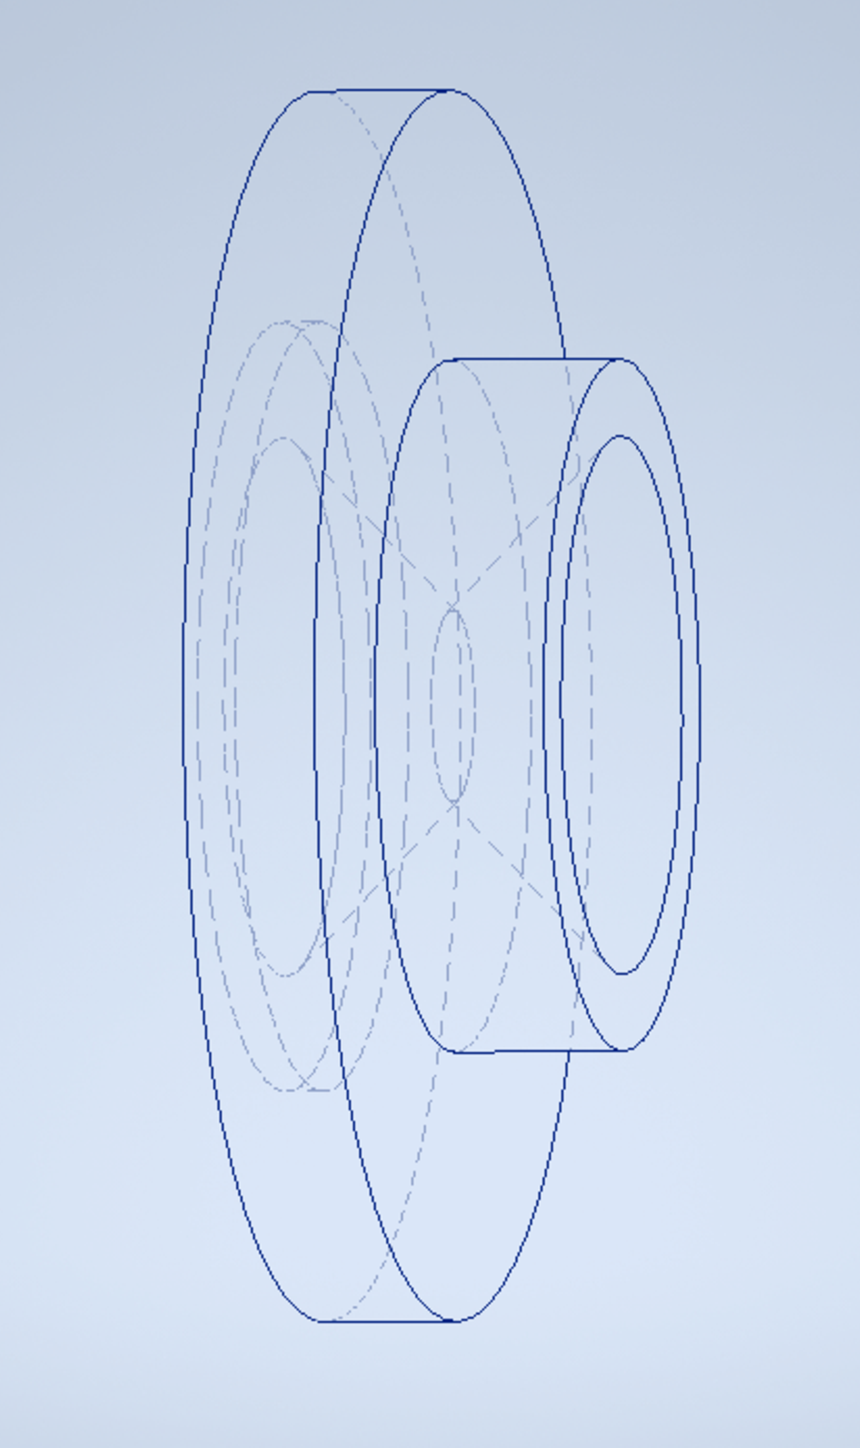
\includegraphics[scale=0.2]{newchamfer.pdf}
        \caption{Old vs New Chamfer Geometry}
    \end{figure}
\end{frame}
\begin{frame}[allowframebreaks]{References}
    \bibliography{demo}
    \bibliographystyle{elsarticle-num}
  
  \end{frame}
\end{document}